\documentclass{beamer}

% xcolor and define colors -------------------------
\usepackage{xcolor}

% https://www.viget.com/articles/color-contrast/
\definecolor{purple}{HTML}{5601A4}
\definecolor{navy}{HTML}{0D3D56}
\definecolor{ruby}{HTML}{9a2515}
\definecolor{alice}{HTML}{107895}
\definecolor{daisy}{HTML}{EBC944}
\definecolor{coral}{HTML}{F26D21}
\definecolor{kelly}{HTML}{829356}
\definecolor{cranberry}{HTML}{E64173}
\definecolor{jet}{HTML}{131516}
\definecolor{asher}{HTML}{555F61}
\definecolor{slate}{HTML}{314F4F}

% Mixtape Sessions
\definecolor{picton-blue}{HTML}{00b7ff}
\definecolor{violet-red}{HTML}{ff3881}
\definecolor{sun}{HTML}{ffaf18}
\definecolor{electric-violet}{HTML}{871EFF}

% Main theme colors
\definecolor{accent}{HTML}{00b7ff}
\definecolor{accent2}{HTML}{871EFF}
\definecolor{gray100}{HTML}{f3f4f6}
\definecolor{gray800}{HTML}{1F292D}


% Beamer Options -------------------------------------

% Background
\setbeamercolor{background canvas}{bg = white}

% Change text margins
\setbeamersize{text margin left = 15pt, text margin right = 15pt} 

% \alert
\setbeamercolor{alerted text}{fg = accent2}

% Frame title
\setbeamercolor{frametitle}{bg = white, fg = jet}
\setbeamercolor{framesubtitle}{bg = white, fg = accent}
\setbeamerfont{framesubtitle}{size = \small, shape = \itshape}

% Block
\setbeamercolor{block title}{fg = white, bg = accent2}
\setbeamercolor{block body}{fg = gray800, bg = gray100}

% Title page
\setbeamercolor{title}{fg = gray800}
\setbeamercolor{subtitle}{fg = accent}

%% Custom \maketitle and \titlepage
\setbeamertemplate{title page}
{
    %\begin{centering}
        \vspace{20mm}
        {\Large \usebeamerfont{title}\usebeamercolor[fg]{title}\inserttitle}\\
        {\large \itshape \usebeamerfont{subtitle}\usebeamercolor[fg]{subtitle}\insertsubtitle}\\ \vspace{10mm}
        {\insertauthor}\\
        {\color{asher}\small{\insertdate}}\\
    %\end{centering}
}

% Table of Contents
\setbeamercolor{section in toc}{fg = accent!70!jet}
\setbeamercolor{subsection in toc}{fg = jet}

% Button 
\setbeamercolor{button}{bg = accent}

% Remove navigation symbols
\setbeamertemplate{navigation symbols}{}

% Table and Figure captions
\setbeamercolor{caption}{fg=jet!70!white}
\setbeamercolor{caption name}{fg=jet}
\setbeamerfont{caption name}{shape = \itshape}

% Bullet points

%% Fix left-margins
\settowidth{\leftmargini}{\usebeamertemplate{itemize item}}
\addtolength{\leftmargini}{\labelsep}

%% enumerate item color
\setbeamercolor{enumerate item}{fg = accent}
\setbeamerfont{enumerate item}{size = \small}
\setbeamertemplate{enumerate item}{\insertenumlabel.}

%% itemize
\setbeamercolor{itemize item}{fg = accent!70!white}
\setbeamerfont{itemize item}{size = \small}
\setbeamertemplate{itemize item}[circle]

%% right arrow for subitems
\setbeamercolor{itemize subitem}{fg = accent!60!white}
\setbeamerfont{itemize subitem}{size = \small}
\setbeamertemplate{itemize subitem}{$\rightarrow$}

\setbeamertemplate{itemize subsubitem}[square]
\setbeamercolor{itemize subsubitem}{fg = jet}
\setbeamerfont{itemize subsubitem}{size = \small}


% Special characters

\usepackage{collectbox}

\makeatletter
\newcommand{\mybox}{%
    \collectbox{%
        \setlength{\fboxsep}{1pt}%
        \fbox{\BOXCONTENT}%
    }%
}
\makeatother





% Links ----------------------------------------------

\usepackage{hyperref}
\hypersetup{
  colorlinks = true,
  linkcolor = accent2,
  filecolor = accent2,
  urlcolor = accent2,
  citecolor = accent2,
}


% Line spacing --------------------------------------
\usepackage{setspace}
\setstretch{1.1}


% \begin{columns} -----------------------------------
\usepackage{multicol}


% Fonts ---------------------------------------------
% Beamer Option to use custom fonts
\usefonttheme{professionalfonts}

% \usepackage[utopia, smallerops, varg]{newtxmath}
% \usepackage{utopia}
\usepackage[sfdefault,light]{roboto}

% Small adjustments to text kerning
\usepackage{microtype}



% Remove annoying over-full box warnings -----------
\vfuzz2pt 
\hfuzz2pt


% Table of Contents with Sections
\setbeamerfont{myTOC}{series=\bfseries, size=\Large}
\AtBeginSection[]{
        \frame{
            \frametitle{Roadmap}
            \tableofcontents[current]   
        }
    }


% Tables -------------------------------------------
% Tables too big
% \begin{adjustbox}{width = 1.2\textwidth, center}
\usepackage{adjustbox}
\usepackage{array}
\usepackage{threeparttable, booktabs, adjustbox}
    
% Fix \input with tables
% \input fails when \\ is at end of external .tex file
\makeatletter
\let\input\@@input
\makeatother

% Tables too narrow
% \begin{tabularx}{\linewidth}{cols}
% col-types: X - center, L - left, R -right
% Relative scale: >{\hsize=.8\hsize}X/L/R
\usepackage{tabularx}
\newcolumntype{L}{>{\raggedright\arraybackslash}X}
\newcolumntype{R}{>{\raggedleft\arraybackslash}X}
\newcolumntype{C}{>{\centering\arraybackslash}X}

% Figures

% \imageframe{img_name} -----------------------------
% from https://github.com/mattjetwell/cousteau
\newcommand{\imageframe}[1]{%
    \begin{frame}[plain]
        \begin{tikzpicture}[remember picture, overlay]
            \node[at = (current page.center), xshift = 0cm] (cover) {%
                \includegraphics[keepaspectratio, width=\paperwidth, height=\paperheight]{#1}
            };
        \end{tikzpicture}
    \end{frame}%
}

% subfigures
\usepackage{subfigure}


% Highlight slide -----------------------------------
% \begin{transitionframe} Text \end{transitionframe}
% from paulgp's beamer tips
\newenvironment{transitionframe}{
    \setbeamercolor{background canvas}{bg=accent!40!black}
    \begin{frame}\color{accent!10!white}\LARGE\centering
}{
    \end{frame}
}


% Table Highlighting --------------------------------
% Create top-left and bottom-right markets in tabular cells with a unique matching id and these commands will outline those cells
\usepackage[beamer,customcolors]{hf-tikz}
\usetikzlibrary{calc}
\usetikzlibrary{fit,shapes.misc}

% To set the hypothesis highlighting boxes red.
\newcommand\marktopleft[1]{%
    \tikz[overlay,remember picture] 
        \node (marker-#1-a) at (0,1.5ex) {};%
}
\newcommand\markbottomright[1]{%
    \tikz[overlay,remember picture] 
        \node (marker-#1-b) at (0,0) {};%
    \tikz[accent!80!jet, ultra thick, overlay, remember picture, inner sep=4pt]
        \node[draw, rectangle, fit=(marker-#1-a.center) (marker-#1-b.center)] {};%
}

\usepackage{breqn} % Breaks lines

\usepackage{amsmath}
\usepackage{mathtools}

\usepackage{pdfpages} % \includepdf

\usepackage{listings} % R code
\usepackage{verbatim} % verbatim

% Video stuff
\usepackage{media9}

% packages for bibs and cites
\usepackage{natbib}
\usepackage{har2nat}
\newcommand{\possessivecite}[1]{\citeauthor{#1}'s \citeyearpar{#1}}
\usepackage{breakcites}
\usepackage{alltt}

% Setup math operators
\DeclareMathOperator{\E}{E} \DeclareMathOperator{\tr}{tr} \DeclareMathOperator{\se}{se} \DeclareMathOperator{\I}{I} \DeclareMathOperator{\sign}{sign} \DeclareMathOperator{\supp}{supp} \DeclareMathOperator{\plim}{plim}
\DeclareMathOperator*{\dlim}{\mathnormal{d}\mkern2mu-lim}
\newcommand\independent{\protect\mathpalette{\protect\independenT}{\perp}}
   \def\independenT#1#2{\mathrel{\rlap{$#1#2$}\mkern2mu{#1#2}}}
\newcommand*\colvec[1]{\begin{pmatrix}#1\end{pmatrix}}

\newcommand{\myurlshort}[2]{\href{#1}{\textcolor{gray}{\textsf{#2}}}}


\begin{document}

\imageframe{./lecture_includes/mixtape_did_cover.png}


% ---- Content ----

\section{Difference-in-Differences}

\subsection{Origins}


\begin{frame}{Introduction}

\begin{itemize}
\item Scott Cunningham, Ben H. Williams Professor of Economics at Baylor University in Texas USA
\item Wanted to walk you through the history of diff-in-diff
\item Will show you stories, pictures, and code
\end{itemize}

\end{frame}





\begin{frame}{Diff-in-diff popularity}

	\begin{figure}
	\caption{Currie, et al. (2020)}
	\includegraphics[scale=0.25]{./lecture_includes/currie_did.png}
	\end{figure}

\end{frame}









\begin{frame}{What is difference-in-differences (DiD)}

\begin{itemize}
\item DiD is when a group of units are assigned some treatment and then compared to a group of units that weren't before and after
\item One of the most widely used quasi-experimental methods in economics and increasingly in industry
\item Predates the randomized experiment by 80 years, but uses basic experimental ideas about treatment and control groups (just not randomized)
\item Uses panel or repeated cross section datasets, binary treatments usually, and often covariates
\item We'll do a quick run through the social history of diff-in-diff to set the stage for our workshop this week
\end{itemize}
\end{frame}








\begin{frame}{Ignaz Semmelweis and washing hands}

\begin{itemize}
\item Early 1820s, Vienna passed legislation requiring that if a pregnant women giving birth went to a public hospital (free care), then depending on the day of week and time of day, she would be routed to either the midwife wing or the physician wing (most likely resulting in random assignment)
\item But by the 1840s, Ignaz Semmelweis noticed that pregnant women died after delivery in the (male) wing at a rate of 13-18\%, but only 3\% in the (female) midwife wing -- cause was puerperal or “childbed” fever
\item Somehow this was also we known -- women would give birth in the street rather than go to the physician if they were unlucky enough to have their water break on the wrong day and time
\end{itemize}

\end{frame}

\begin{frame}{Ignaz Semmelweis and washing hands}

\begin{itemize}
\item Ignaz Semmelweis conjectures after a lot of observation that the cause is the teaching faculty teaching anatomy using cadavers and then delivering babies \emph{without washing hands}
\item New training happens to one but not the other and Semmelweis thinks the mortality is caused by working with cadavers
\item Convinced the hospital to have physicians wash their hands in chlorine but not the midwives, creating a type of difference-in-differences design 
\end{itemize}

\end{frame}

\begin{frame}{Semmelweis diff-in-diff evidence}

	\begin{figure}
	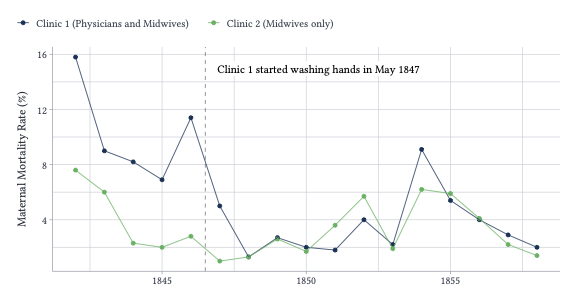
\includegraphics[scale=0.5]{./lecture_includes/semmelweis_raw_plots}
	\end{figure}


\end{frame}

\begin{frame}{Evidence Rejected}

\begin{itemize}

\item Diff-in-diff evidence was rejected by Semmelweis' superiors claiming it was the hospital's new ventilation system
\item Dominant theory of disease spread was caused by "odors" or miasma or "humors"
\item Semmelweis began showing signs of irritability, perhaps onset of dementia, became publicly abusive, was committed to a mental hospital and within two weeks died from wounds he received while in residence
\item Despite the strength of evidence, difference-in-differences was rejected -- a theme we will see continue

\end{itemize}

\end{frame}






\begin{frame}{John Snow and cholera}

\begin{itemize}
\item Three major waves of cholera in the early to mid 1800s in London, largely thought to be spread by miasma (``dirty air'')
\item John Snow believed cholera was spread through the Thames water supply through an invisible creature that entered the body through food and drink, caused the body to expel water, placing the creature back in the Thames and causing epidemic waves
\item London passes ordinance requiring water utility companies to move inlet pipe further up the Thames, above the city center, but not everyone complies
\item Natural experiment: Lambeth water company moves its pipe between 1849 and 1854; Southwark and Vauxhall water company delayed
\end{itemize}

\end{frame}


\begin{frame}

	\begin{figure}
	\caption{Two water utility companies in London 1854}
	\includegraphics[scale=0.225]{./lecture_includes/lambeth.png}
	\end{figure}


\end{frame}



\begin{frame}{Difference-in-differences}

\begin{table}\centering
\scriptsize
		\caption{Lambeth and Southwark and Vauxhall, 1849 and 1854}
		\begin{center}
		\begin{tabular}{lll|lc}
		\toprule
		\multicolumn{1}{l}{\textbf{Companies}}&
		\multicolumn{1}{c}{\textbf{Time}}&
		\multicolumn{1}{c}{\textbf{Outcome}}&
		\multicolumn{1}{c}{$D_1$}&
		\multicolumn{1}{c}{$D_2$}\\
		\midrule
		Lambeth & Before & $Y=L$ \\
		& After & $Y=L + L_t + D$ & $\textcolor{red}{L_t}+D$\\
		\midrule
		& & & & $D + (\textcolor{red}{L_t}- SV_t)$ \\
		\midrule
		Southwark and Vauxhall & Before & $Y=SV$ \\
		& After & $Y=SV + SV_t$ & $SV_t$\\
		\bottomrule
		\end{tabular}
		\end{center}
	\end{table}

\begin{eqnarray*}
\widehat{\delta}_{did} = D + (\textcolor{red}{L_t}- SV_t)
\end{eqnarray*}This method yields an unbiased estimate of D if $\textcolor{red}{L_t} = SV_t$, but note that $\textcolor{red}{L_t}$ is a counterfactual trend and therefore not known

\end{frame}


\begin{frame}
\begin{center}
\textbf{Two rivers into causal inference}
\end{center}

\begin{tikzpicture}[scale=0.7, every node/.style={scale=0.7}]
% Orley Ashenfelter Stream
\node at (-5,6) {\textbf{Orley Ashenfelter}};
\draw[->, thick] (-5,5.5) -- (-5,5.2);
\node at (-5,5) {Princeton Industrial Relations Section};
\draw[->, thick] (-5,4.5) -- (-5,4.2);
\node at (-5,4) {Quasi-Experimental Design};
\draw[->, thick] (-5,3.5) -- (-5,3.2);
\node at (-5,3) {David Card};
\draw[->, thick] (-5,2.5) -- (-5,2.2);
\node at (-5,2) {Alan Krueger};
\draw[->, thick] (-5,1.5) -- (-5,1.2);

% Don Rubin Stream
\node at (5,6) {\textbf{Don Rubin}};
\draw[->, thick] (5,5.5) -- (5,5.2);
\node at (5,5) {Harvard Statistics};
\draw[->, thick] (5,4.5) -- (5,4.2);
\node at (5,4) {Experimental Design};
\draw[->, thick] (5,3.5) -- (5,3.2);
\node at (5,3) {Potential Outcomes};
\draw[->, thick] (5,2.5) -- (5,2.2);
\node at (5,2) {Treatment Effects};
\draw[->, thick] (5,1.5) -- (5,1.2);

% Arrow from Orley Ashenfelter and Don Rubin streams to bottom rectangle
\draw[->, thick] (-5,1) -- (0,-0.8);
\draw[->, thick] (5,1) -- (0,-0.8);

% Bottom Rectangle
\node[draw, minimum width=8cm, minimum height=2cm, anchor=north] at (0,-0.8) {
    \begin{tabular}{c}
        Josh Angrist \\
        (Princeton)
    \end{tabular}
    \hspace{2cm}
    \begin{tabular}{c}
        Guido Imbens \\
        (Brown)
    \end{tabular}
};
\node[anchor=north] at (0,-2.8) {\textbf{Harvard Economics}};

\end{tikzpicture}

\end{frame}


\begin{frame}{Background I: Harvard Stats and Potential Outcomes}
  \begin{itemize}
    \item Don Rubin, former chair of Harvard stats, is the main source of potential outcomes, building on Jerzy Neyman's 1923 work.
    \item Rubin's influential 1970s papers advocated for causal inference using contrasts of $Y(1)$ and $Y(0)$.
    \item Neyman's notation, initially in Polish, was translated into English in 1990, likely due to Rubin.
    \item Rubin expanded Neyman's ideas from experiments to observational studies, leading to developments like propensity score methods.
    \item Economics was slow to adopt these methods initially.
  \end{itemize}
\end{frame}


\begin{frame}{Background II: Princeton Industrial Relations Section}
  \begin{itemize}
    \item Late 1970s and early 1980s: little "credibility" in empirical labor studies.
    \item Princeton Industrial Relations Section: older than the economics dept, rigorous, non-partisan focus on US "manpower", highly empirical.
    \item Key faculty are Orley Ashenfelter, David Card, Alan Krueger.
    \item Key students include Bob Lalonde, Josh Angrist, Steve Pischke, John Dinardo, Janet Currie, Anne Case, and many more.
    \item Listen to David Card: \url{https://youtu.be/1soLdywFb_Q?si=BCVqYeRz6jYiwHTQ&t=1580}
  \end{itemize}
\end{frame}


\begin{frame}{Background II: Princeton Industrial Relations Section}
Example of Princeton Paradigm Emerging
  \begin{itemize}
    \item Lalonde (1986) was a groundbreaking study, recently reviewed by Guido Imbens and Yiqing Xu (2024)
    \item Lalonde, a student of Card and Orley, analyzed an RCT on a job training program, finding an average treatment effect of +\$800.
    \item He then replaced the experimental control group with survey data, reran econometric methods, and couldn't replicate the results.
    \item Orley and Card emphasized randomization in their 1985 Restat article, advocating for its exploitation in studies.
  \end{itemize}
\end{frame}


\begin{frame}{Orley Ashenfelter and diff-in-diff}

\begin{itemize}

\item Diff-in-diff gets rediscovered by Orley Ashenfelter from Princeton 
\item Leaves academia to work in Washington DC to study job training programs for low skill workers
\item Coins the phrase "difference-in-differences" so as to avoid having to explain regressions to bureaucrats (3:53)  \url{https://youtu.be/WnB3EJ8K7lg?si=uE4clqUIPzvbxm0r&t=2}
\item More associated with David Card (Mariel boatlift, minimum wage), but it was earlier that he and Orley worked with the method, and ironically largely, rejected its usefulness for the questions they were working on

\end{itemize}

\end{frame}





\begin{frame}{Minimum wages}

\begin{itemize}
\item Card and Krueger (1994) have a famous study estimating causal effect of minimum wages on employment
\item  New Jersey raises its minimum wage in April 1992 (between February and November) but neighboring Pennsylvania does not
\item Using DiD, they do not find a negative effect of the minimum wage on employment leading to complex reactions from economists
\item Orley's describes his understanding of people's reaction to the paper.  \\ \url{https://youtu.be/MOtbuRX4eyQ?t=1882}
\end{itemize}

\end{frame}

\begin{frame}
	\begin{figure}
	\includegraphics[scale=0.5]{./lecture_includes/minwage_whore}
	\end{figure}
\end{frame}


\begin{frame}{Reaction to the paper}


Lots of anecdotes in this interview with Card, but here are just two.  First, Card and Krueger received a lot of personal hostility from their peers (1:07 to 1:10)

\bigskip

\url{https://youtu.be/1soLdywFb_Q?si=laAVYf_E2KBZKywG&t=4020}

\bigskip

Later Card says Sherwin Rosen accused them of having an agenda.  But the worst is what happens to Alan Krueger maybe (1:16 to 1:17)

\bigskip

\url{https://youtu.be/1soLdywFb_Q?si=jsb8h50ZosGDnKrv&t=4556}




\end{frame}

\begin{frame}{Card on that study}

\begin{quote}
``I’ve subsequently stayed away from the minimum wage literature for a number of reasons. First, it cost me a lot of friends. People that I had known for many years, for instance, some of the ones I met at my first job at the University of Chicago, became very angry or disappointed. They thought that in publishing our work we were being traitors to the cause of economics as a whole.''
\end{quote}


\end{frame}



\begin{frame}{OLS specification of the DiD equation}
	
	\begin{itemize}
	\item The correctly specified OLS regression is an interaction with time and group fixed effects:$$Y_{its} = \alpha + \gamma NJ_s + \lambda d_t + \delta (NJ \times d)_{st} + \varepsilon_{its}$$
		\begin{itemize}
		\item NJ is a dummy equal to 1 if the observation is from NJ
		\item d is a dummy equal to 1 if the observation is from November (the post period)
		\end{itemize}
	\item This equation takes the following values
		\begin{itemize}
		\item PA Pre: $\alpha$
		\item PA Post: $\alpha + \lambda$
		\item NJ Pre: $\alpha + \gamma$
		\item NJ Post: $\alpha + \gamma + \lambda + \delta$
		\end{itemize}
	\item DiD equation: (NJ Post - NJ Pre) - (PA Post - PA Pre) $= \delta$
	\end{itemize}
\end{frame}




\begin{frame}[plain]
	$$Y_{ist} = \alpha + \gamma NJ_s + \lambda d_t + \delta(NJ\times d)_{st} + \varepsilon_{ist}$$
	\begin{figure}
	\includegraphics[scale=0.90]{./lecture_includes/waldinger_dd_5.pdf}
	\end{figure}
\end{frame}


\begin{frame}[plain]
	$$Y_{ist} = \alpha + \gamma NJ_s + \lambda d_t + \delta(NJ\times d)_{st} + \varepsilon_{ist}$$
	\begin{figure}
	\includegraphics[scale=0.90]{./lecture_includes/waldinger_dd_5.pdf}
	\end{figure}

Notice how OLS is ``imputing'' $E[Y^0|D=1,Post]$ for the treatment group in the post period? It is only ``correct'', though, if parallel trends is a good approximation

\end{frame}





\section{Parallel Trends Violations}

\subsection{Results versus Evidence}



\begin{frame}{Evidence versus the Main Result}

\begin{itemize}
\item Causal inference is about \emph{warranted beliefs} -- should you or should you not believe the \emph{causal claim}?
\item Your DiD \emph{results} are like the claim of guilt, but your DiD results are \emph{not} the smoking gun
	\begin{itemize}
	\item Your table of regression coefficients \emph{is not enough} for evidence
	\item You need to do more to provide a justification for parallel trends
	\end{itemize}
\item You need to provide evidence for parallel trends against several well known vulnerabilities
\item Evidence will be bite, falsifications, mechanisms and event study data visualization 
\item We will mix the parallel trends violations with the evidence concept before getting into advanced estimators
\end{itemize}

\end{frame}


\begin{frame}{Court metaphor}

	\begin{itemize}
	\item Think of yourself as a prosecutor arguing against a defense attorney to convince a judge and jury of a defendant's guilt
	\item The claim the defendant is guilty is your table of main results
	\item But the claim is not the evidence -- you have to back up that claim 
	\item Your evidence of guilt is the smoking gun, the fingerprints, the eye witnesses, the footprints in the mud outside the house
	\item If your claim is supported by weak evidence, then no one \emph{should} convict -- it would be borderline corruption if they did 
	\end{itemize}

\end{frame}



\begin{frame}{Event study regression}
	
	\begin{itemize}
	\item Alternatively, present estimated coefficients from a dynamic regression specification:
 $$Y_{its} = \alpha + \sum_{\tau=-2}^{-q}\mu_{\tau} (D_s \times \tau_t) + \sum_{\tau=0}^m\delta_{\tau} (D_s \times \tau_t) + \tau_t + D_s + \varepsilon_{ist}$$
		\begin{itemize}
		\item With a simple 2x2, you are interacting treatment indicator with calendar year dummies
		\item Includes $q$ leads (dropping the $t-1$ as baseline) and $m$ lags 
		\item Since treatment did not happen until $\tau=0$, then pre-treatment coefficients only capture differential trends
		\end{itemize}
	\item Estimated $\widehat{\delta}_\tau$ coefficients are estimated ATT for each year under parallel trends but $\widehat{\mu}_\tau$ is your smoking gun evidence 
	\item Just remember that $\mu=0$ is not the same as parallel trends as parallel trends is \textcolor{red}{untestable}.
	\end{itemize}
\end{frame}

\begin{frame}{Reviewing previous slide for emphasis}


\begin{itemize}
\item Under NA, SUTVA and parallel pre-trends, then mechanically $\widehat{\mu_{\tau}}$ will be zero as everything cancels out
	\begin{itemize}
\item There are still specification and power issues that Jon Roth has written about, but I will skip that
	\end{itemize}
\item But also under NA, SUTVA and parallel trends (post trends), then $\widehat{\delta}$ are estimates of the ATT at points in time
\item  Typically you'll plot the coefficients and 95\% CI on all leads and lags
\end{itemize}

\end{frame}

\begin{frame}{DiD coefficient}

$$\delta = \text{ATT} + \text{Non-Parallel Trends Bias}$$

You want to know if trends would've been the same had the policy not happened. 


\end{frame}

\begin{frame}{Pre-treatment DiD coefficient}

\begin{eqnarray*}
\widehat{\delta}_{t-2} &=& \bigg [  \underbrace{\textcolor{black}{E[Y^0_k | t-2]} - E[Y^0_k | t-1] \bigg ] - \bigg [ E[Y^0_U | t-2] - E[Y_U^0 | t-1] }_{\mathclap{\text{Non-parallel trends bias in 2x2 case}}} \bigg ]
\end{eqnarray*}

\bigskip

Under NA, then the $t-1$ period is untreated.  But then so are the other pre-periods so the ATT is implicitly zero and the \emph{only} thing that you can be measuring with pre-trend DiD coefficients is differential trends.  


\end{frame}



\begin{frame}{Event study coefficients}

\begin{itemize}
\item Remember that the OLS specification we discuss collapses to ATT plus parallel trends bias
\item This is \emph{always} true because it's an identity and holds even in the pre-period as much in the post
\item It's just in the pre period, you do not have the missing $E[Y^0|D=1]$ term as no one and nothing is treated in pre-period under NA
\item This means pre-period is basically an opportunity to directly verify parallel pre-trends -- but it's the past's pre-trends, not the counterfactual pre-trend of the present/future
\item And that's how people use the pre-period -- they use the pre-period to evaluate whether they think this is a good control group
\end{itemize}

\end{frame}

\begin{frame}{Event study example}

\begin{itemize}
\item The notion is really simple: if PT held then, you'll argue that it's reasonable it would've still held
\item But this is an assertion, and you need to build the case as we said
\item At this point, it's a lot easier to show you what I'm talking about -- where the art and the science meet -- with a great paper
\end{itemize}

\end{frame}




\begin{frame}{Medicaid and Affordable Care Act example}

\begin{figure}
\includegraphics[scale=0.25]{./lecture_includes/medicaid_qje}
\end{figure}

\end{frame}
\begin{frame}{Their Evidence versus Their Result}

\begin{itemize}
\item \textbf{Bite} -- they will show that the expansion shifted people into Medicaid and out of uninsured status
\item \textcolor{black}{\textbf{Placebos}} -- they show that there's no effect of Medicaid on a similar group that didn't enroll
\item \textbf{Event study} -- they will lean hard on those dynamic plots
\item \textcolor{red}{\textbf{Main results}} -- with all of this, they will show Medicaid expansion caused near elderly mortality to fall
\item \textcolor{black}{\textbf{Mechanisms}} -- they think they can show it's coming from people treating diseases causing mortality declines to compound over time
\end{itemize}

\end{frame}

\begin{frame}{Bite}

\begin{itemize}
\item Bite is a labor economist's phrase, often used with the minimum wage, to say that the minimum wage actually was binding in the first place
\item Here it means when US states made Medicaid more generous, people got on Medicaid who would not have been on it otherwise
\item And as a bonus, would not have been insured at all without it
\item Not the most exciting result, but imagine if the main results on mortality were shown but there was no evidence for bite -- is it believable?
\end{itemize}

\end{frame}


\imageframe{./lecture_includes/Miller_Medicaid1.png}

\imageframe{./lecture_includes/Miller_Medicaid2.png}

\imageframe{./lecture_includes/Miller_Medicaid3.png}


\begin{frame}{Falsification}

\begin{itemize}

\item Their study focuses on ``near elderly'', which means just under 65
\item They choose just under 65 because in the US, 65 and older are eligible for Medicare so more generous Medicaid is irrelevant
\item \emph{But} probably the near elderly and the elderly are equally susceptible to unobserved factors correlated with the treatment
\item So they painstakingly examine the effects on elderly as a falsification as this will strengthen the parallel trends assumption on the near elderly
\end{itemize}

\end{frame}

\begin{frame}{Falsifications on elderly}

	\begin{figure}
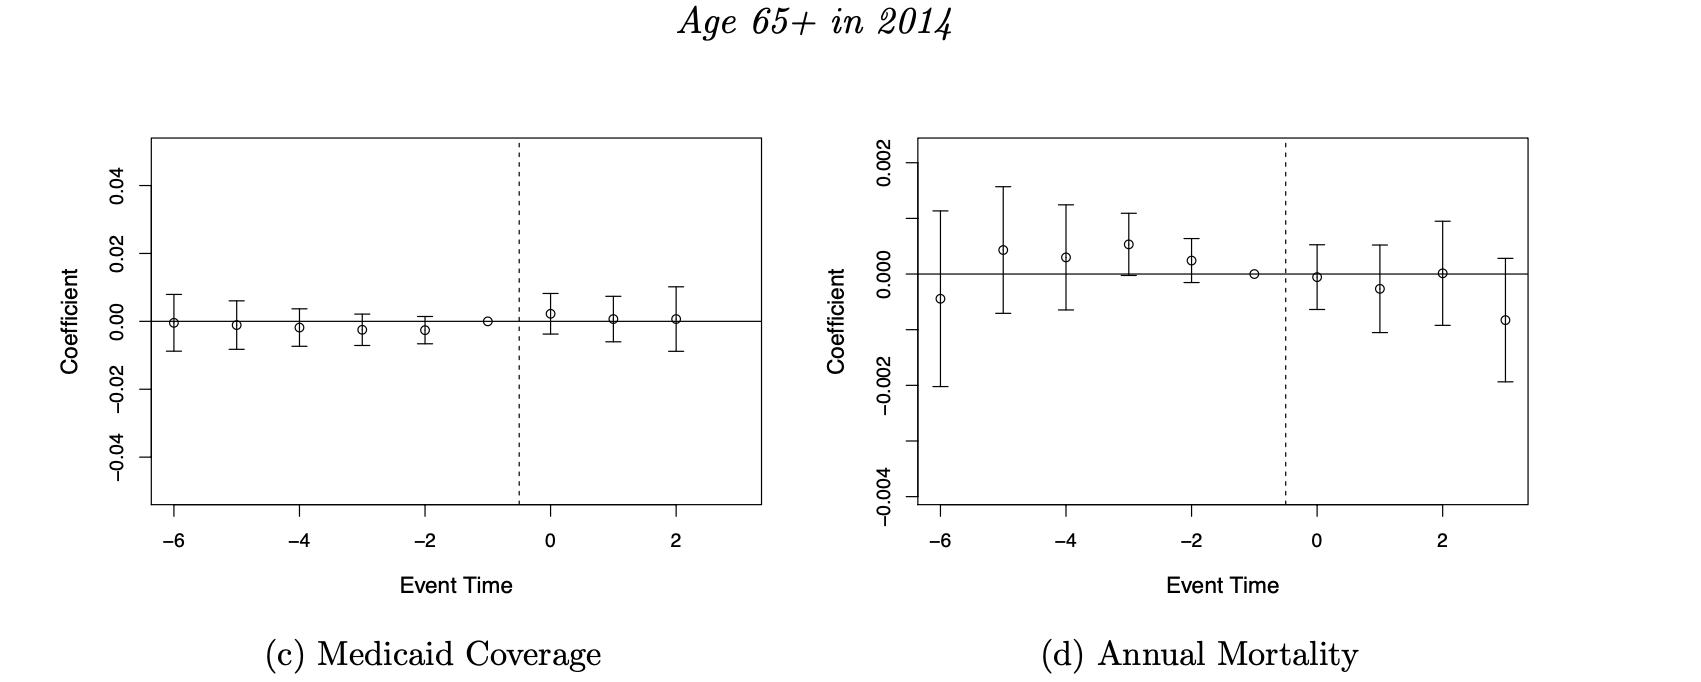
\includegraphics[scale=0.425]{./lecture_includes/placebo_medicaid}
	\end{figure}

\end{frame}

\begin{frame}{Main result}

\begin{itemize}

\item Finally they focus on the main result -- and there's more in the paper than I'm showing
\item Event study plots with same specification as the rest allowing us to look at the pre-trends and the post-treatment coefficients
\item If parallel trends holds, then the post-treatment coefficients are interpreted as ATT parameter estimates for each time period
\item The result alone isn't nearly as strong the result in combination with the rest, but it could still be wrong as parallel trends is ultimately not verfiable
\end{itemize}

\end{frame}



\begin{frame}{Near elderly mortality and Medicaid expansion}

	\begin{figure}
	\includegraphics[scale=0.3]{./lecture_includes/Miller_Medicaid4.png}
	\end{figure}

\end{frame}

\begin{frame}{Summarizing evidence and results}

\begin{itemize}
\item \textbf{Bite}: Increases in enrollment and reductions in uninsured support that there is adoption of the treatment
\item \textbf{Event studies}: Compelling graphics showing similarities between treatment and control
\item \textbf{Falsifications}: no effect on a similar group who isn't eligible
\item \textcolor{red}{Main results}: 9.2\% reduction in mortality among the near-elderly
\item \textcolor{red}{Mechanism}: ``The effect is driven by a reduction in disease-related deaths and grows over time.''
\end{itemize}

\end{frame}

\begin{frame}{Making event study}

\begin{itemize}
\item When there is only one treatment group and one comparison group, then you run a regression with an interaction of the treatment group dummy and the calendar year dummies (plus both separately)
\item You must drop $t-\tau$ as the baseline (e.g., $t-1$) and it must be $Y^0$ untreated comparisons (No Anticipation)
\item I have included in a do file that will do it for you either manually or using coefplot in \texttt{simple\_eventstudy.do} at the shared github labs directory
\end{itemize}

\end{frame}


\begin{frame}{Manually creating the event study}

	\begin{figure}
	\includegraphics[scale=0.20]{./lecture_includes/simple_eventstudy_manual}
	\end{figure}

\end{frame}


\section{Suicides and Prisons}


\begin{frame}{Manually creating the event study}

	\begin{figure}
	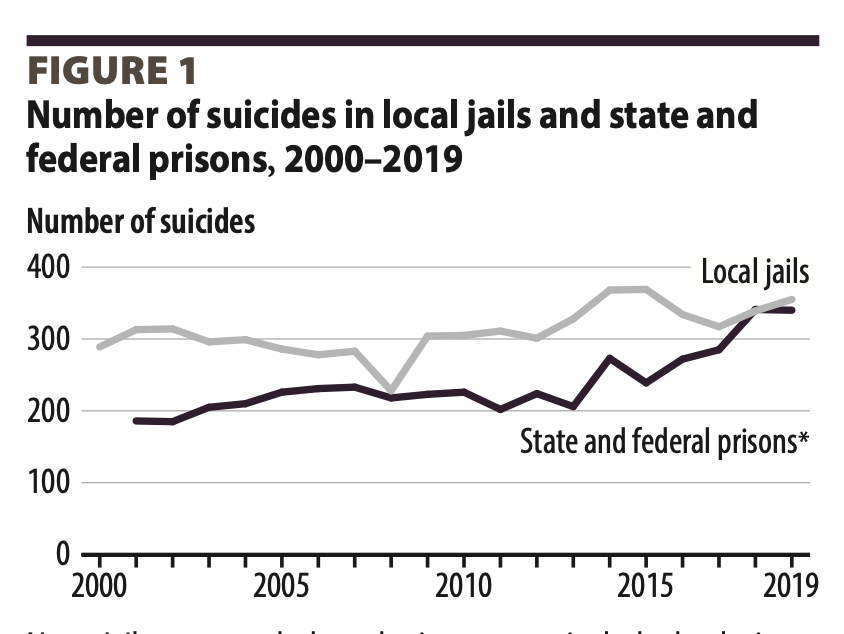
\includegraphics[scale=0.20]{./lecture_includes/bjs_suicides}
	\end{figure}

\end{frame}


\begin{frame}{Suicides and Prisons}

\begin{itemize}

\item Suicide is leading single cause of death in jails
\item From 2001 to 2019, number of suicides in state prisons rose 85\%
\item Texas Dept of Criminal Justice implemented "self harm prevention office" in 15 prisons
\item I'll walk you through some preliminary analysis

\end{itemize}

\end{frame}





\end{document}


